\documentclass[a4paper]{article}

% Packages
\usepackage{graphicx}
\usepackage[margin=1in]{geometry}
\usepackage[backend=bibtex]{biblatex}
\usepackage{comment}
\usepackage{hyperref}


\addbibresource{references.bib}

\title{Evaluation of Machine Translation in Languages}
\author{Stefan Liemawan Adji}
\date{\today}

\begin{document}

\maketitle

\section{Introduction}

Machine translation (MT) is the task of automatically translating from one language to another. This can be done through text or audio. Ideally, machine translation should be able to conserve the contextual, idiomatic and pragmatic nuances of both languages.

Machine translation can be traced down to as early as 1949, \cite{weaver-1999}, with the first public demonstration of an MT system happened on 7th January 1954 through a collaboration with IBM \cite{hutchins-2006-first-mt}. A meticulously chosen set of 49 Russian sentences was translated into English, utilising a highly limited vocabulary of 250 words and only 6 grammar rules. While this had minimal scientific impact, it was impressive enough to encourage substantial funding for MT research in the USA.

The decade of high expectation and disillusion, 1956-1966 \cite{hutchins-2001-mt-50-years}.

The 1960s, particularly 1967-1976 is dubbed as 'the quiet decade' for machine translation by Hutchins \cite{hutchins-2001-mt-50-years}

Rule-based MT relied on extensive linguistic rules and bilingual dictionaries. They were based on syntactic and grammatical rules to parse and generate translations.

Since 1989, the dominance of the rule-based approach has been challenged by the rise of new methods and strategies, collectively referred to as ‘corpus-based’ methods \cite{hutchins-1994-research-methods-mt,hutchins-1998-development-mt}. Subsequently, statistics-based approaches for MT re-emerged, bolstered by the recent success of probabilistic techniques in
speech recognition.

1980s: Statistical Machine Translation (SMT) Emerges, use statistical models, probability

Late 2010s: Rise of Neural Networks
Neural Machine Translation (NMT): Starting around 2014, neural networks began to dominate MT. NMT systems, like those using the sequence-to-sequence (Seq2Seq) model with attention mechanisms (e.g., the Transformer model), demonstrated significant improvements in translation quality.
Advantages Over SMT: NMT models often produce more fluent and coherent translations as they consider the entire sentence context, rather than breaking it down into smaller units like phrases.


...recently growing as a popular research field within Natural Language Processing (NLP). Statistical machine translation \cite{lopez-2008-smt}, which previously dominated for many years in the early 2000s with its reliance on various count-based models, has largely been surpassed by neural machine translation (NMT) in (year). Since the introduction of Transformers in 2017 \cite{vaswani-2017-attention}, Natural Language Processing (NLP) and machine translation in particular reached a giant milestone. The following years saw the birth of Large Language Models (LLMs) such as BERT \cite{devlin-2019-bert} and GPT \cite{openai-2024-gpt4}.

Difference between LLMs and MT engines?
MT engines are specifically designed to translate text from one language to another while preserving the meaning and context as accurately as possible. MT engines can also be based on transformer architectures, but they are usually fine-tuned and optimized for the task of translation. They often incorporate additional components like alignment models and post-processing steps to ensure translation quality.

Primary Function: LLMs focus on generating and understanding natural language text, whereas MT engines focus exclusively on translating text between languages.
Training Data: LLMs are trained on diverse text data from various sources, while MT engines are trained specifically on parallel corpora (texts in two or more languages that are translations of each other).
Output: LLMs generate coherent text in the same language as the input, often in a more creative or conversational style. MT engines produce translated text in a different language, aiming for accuracy and fidelity to the original meaning.

According to Ethnologue \cite{ethnologue-2024}, 7,164 languages currently exist and in use today, with 40\% of them considered endangered.

As of July 2024, 243 languages are supported by Google Translate (according to Wikipedia \cite{wikipedia-google-translate})

Many language models are trained on predominantly English NLP tasks, before fine-tuned for downstream tasks in other languages.

There is little insights on how the current state of machine translation is across different language. Therefore...

There does not seem to be a lot of pre-trained models that focuses on a single language. This could be because multilingual LLMs perform better? find proof

Focus on single-language models?

Through simple experimentation and analysis, this paper aims to evaluate existing techniques across different languages
and contribute valuable insights into the current state of machine translation technology. By comparing metrics among languages, I hope to inform future researchers of the effectiveness of machine translation on each individual languages that are included in this paper.

\section{Literature Review}

DeepL \cite{deepl} is a machine translation service that has gained widespread acclaim, currently proclaimed itself as the world's most accurate translator. There is not much information on how the model or techniques as it is essentially a private business. (irrelevant?)


Instruction Learning and decoder-based models...

GPT \cite{openai-2024-gpt4}

Multilingual Language Models are on the rise for the task of machine translation that involves several languages

A major drawback within most multilingual LMs nowadays is that they are either trained, tested, prioritised on English first.


mBERT \cite{devlin-2019-bert} is the multilingual version of BERT, introduced in the same paper, trained on 104 different languages. However, the model been shown to suffer on low-resource languages \cite{wu-2020-mbert-are-all}.

M-BERT
does create multilingual representations,

T5 \cite{raffel-2023-t5} is a Text-to-Text Transfer Transformer model trained on English.

mt5 \cite{xue-2021-mt5} is a multilingual variant of T5 \cite{raffel-2023-t5}, covering a total of 101 languages.

PolyLM \cite{wei-2023-polylm}

mBart \cite{liu-2020-mbart}

NLLB \cite{nllb200}

MistralAI \cite{jiang-2023-mistral-7b}


Massive Parallel Corpora: The availability of large parallel corpora (datasets containing aligned text pairs in different languages) has been crucial for training effective translation models. Datasets like Europarl, OpenSubtitles, and Common Crawl provide a wealth of parallel text data.
Unsupervised Translation: Techniques have been developed to perform translation without the need for large parallel corpora, using monolingual data to train models that can translate between languages. This is especially useful for low-resource languages.

Multilingual and Zero-Shot Translation:

Multilingual NMT Models: Models like Google's multilingual NMT and Facebook's M2M-100 can translate directly between many language pairs without relying on an intermediate language (like English). These models are trained on datasets containing multiple languages simultaneously.
Zero-Shot Translation: These models can sometimes translate between language pairs they were not explicitly trained on, leveraging knowledge from related languages or shared linguistic features.

\section{Experiments}

\subsection{Dataset}

Tatoeba is a vast, continuously expanding database consisting sentences and their translations, built through the contributions of thousands of volunteers, offering a tool that allows users to see examples of how words are used in sentences \cite{tatoeba}. They currently have 12,132,349 sentences and 423 supported languages, with around one to two thousand new sentences added daily, on average

To build the dataset,

Sentences in English are downloaded, 1,898,494 sentences (it is unclear why it is less than the number stated in the Tatoeba website). Then for each langauges, download sentence pairs compared to English. Merge every language sentences into one big dataframe, only keep where sentences exist for every language

\begin{figure}[htbp]
    \centering
    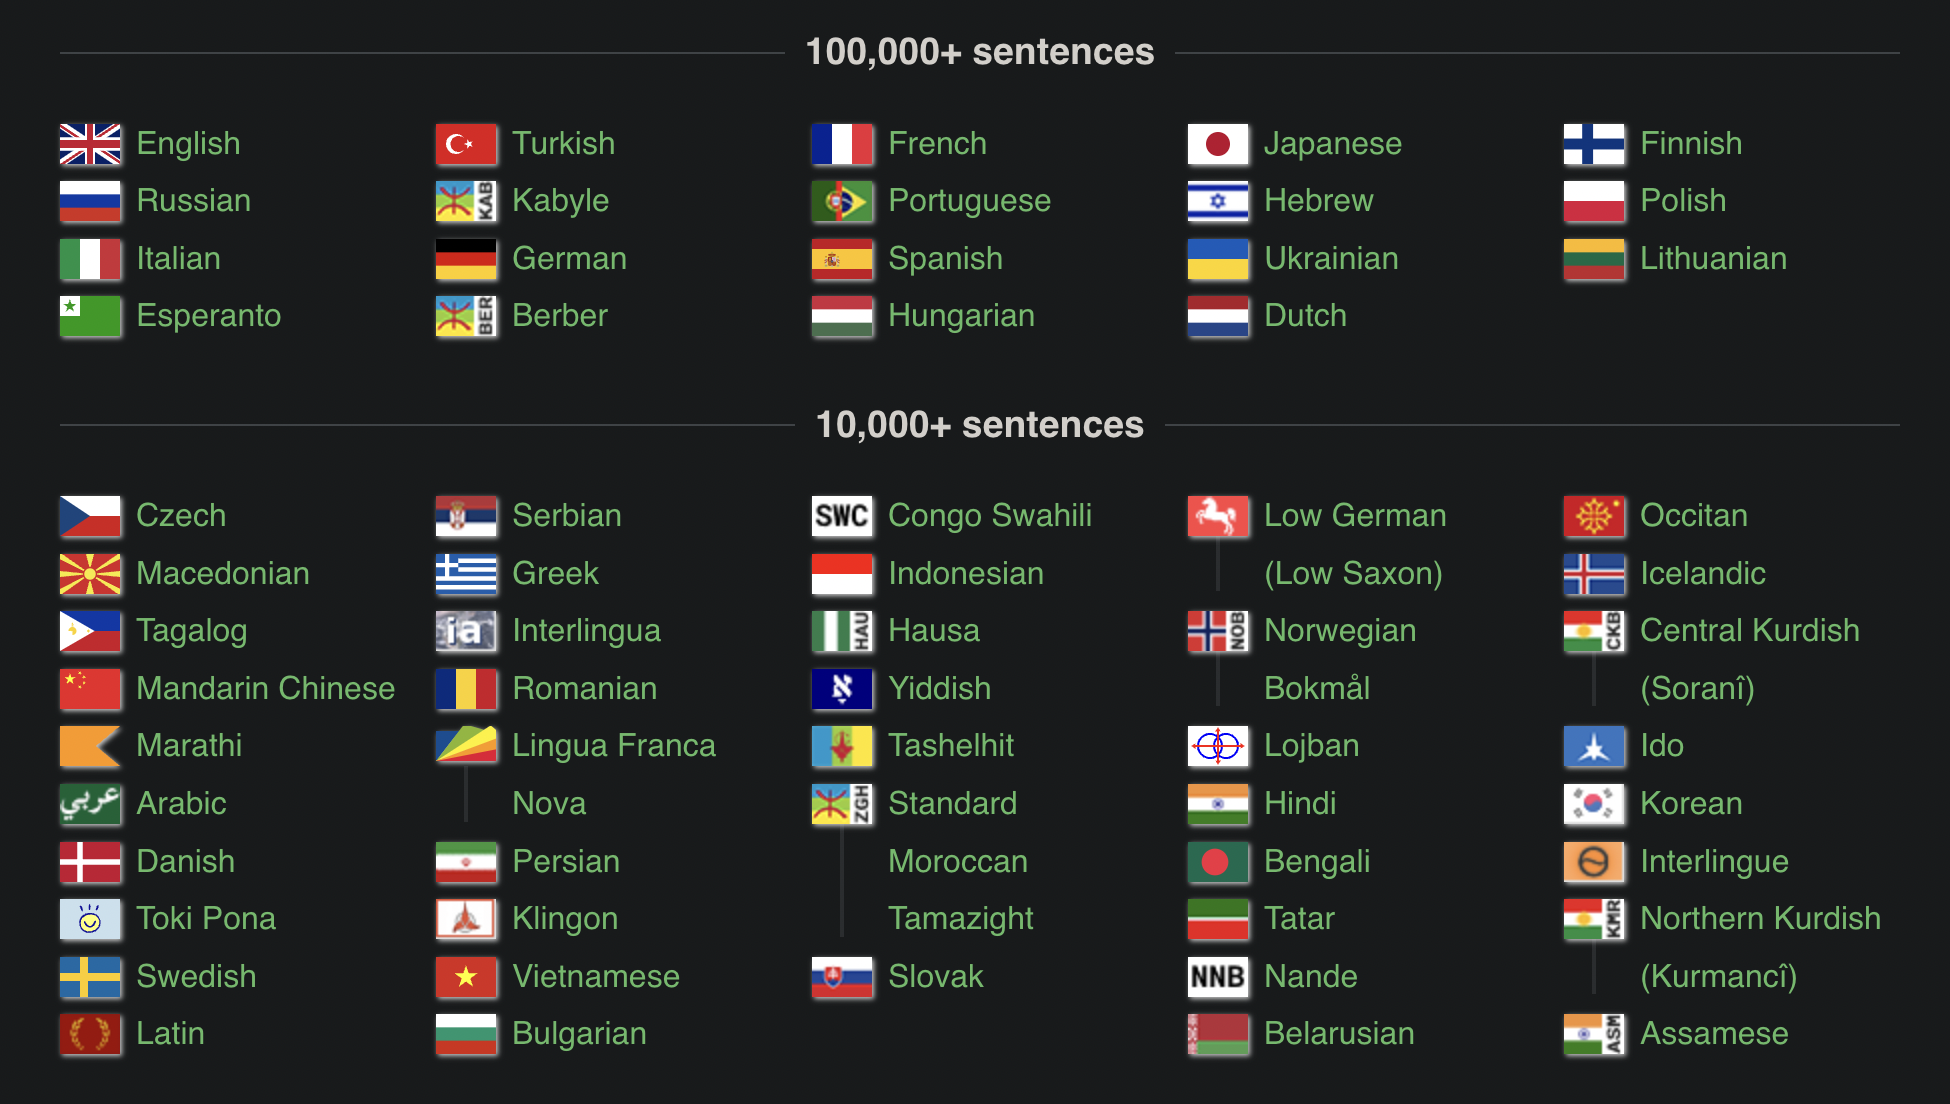
\includegraphics[width=0.9\linewidth]{images/tatoeba_languages.png}
    \caption{Tatoeba languages repository with 10,000+ sentences and 100,000+ sentences \cite{tatoeba}}
    \label{fig:tatoeba_languages}
\end{figure}

Tatoeba English sentence dataset contains 1,905,089 sentences, the largest one in their repository, with Russian in the second place with 1,066,633 sentences. Some of the languages supported in the website is shown in Figure \ref{fig:tatoeba_languages} and Figure \ref{fig:tatoeba_top_bottom_languages}, sorted from the biggest corpus. Low-resource languages such as Rendille, Southern Haida, and Cuyonon can be seen at the bottom of the list, having only a single sentence example. Ancestor languages such as Old Saxon and Old Turkish can also be seen in the list, subsequently with low number of examples.

\begin{figure}[htbp]
    \centering
    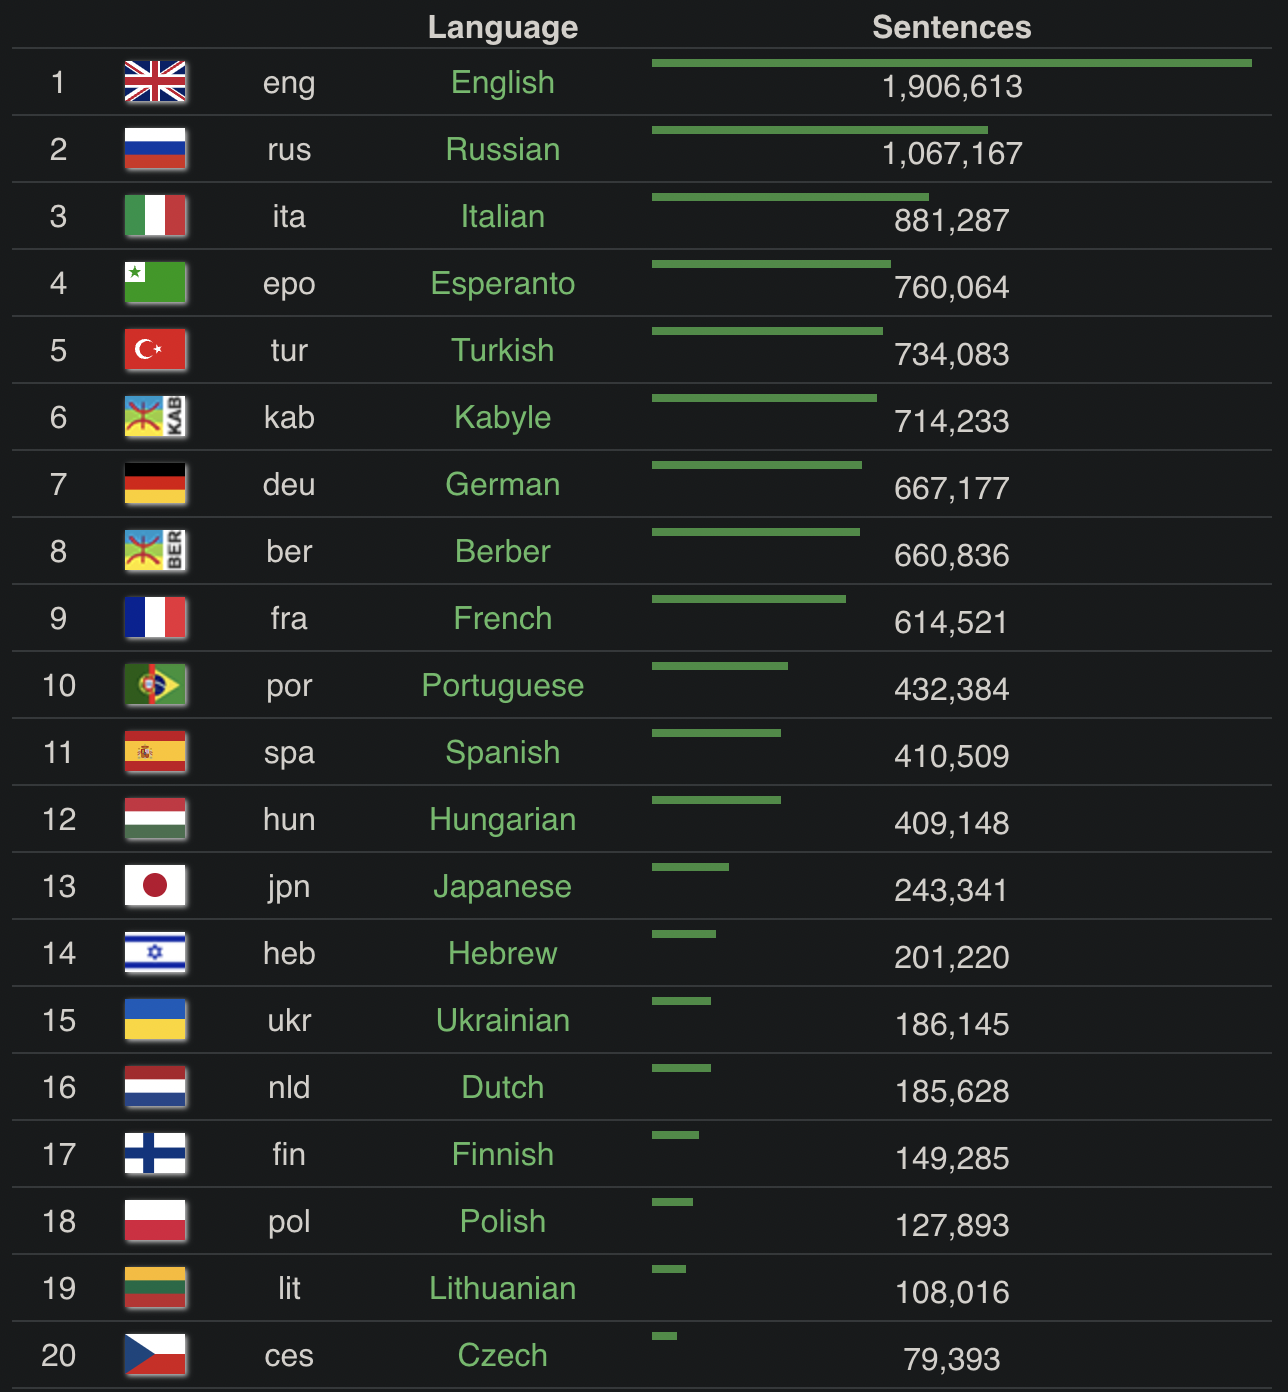
\includegraphics[width=0.5\linewidth]{images/tatoeba_top_20_lang.png}
    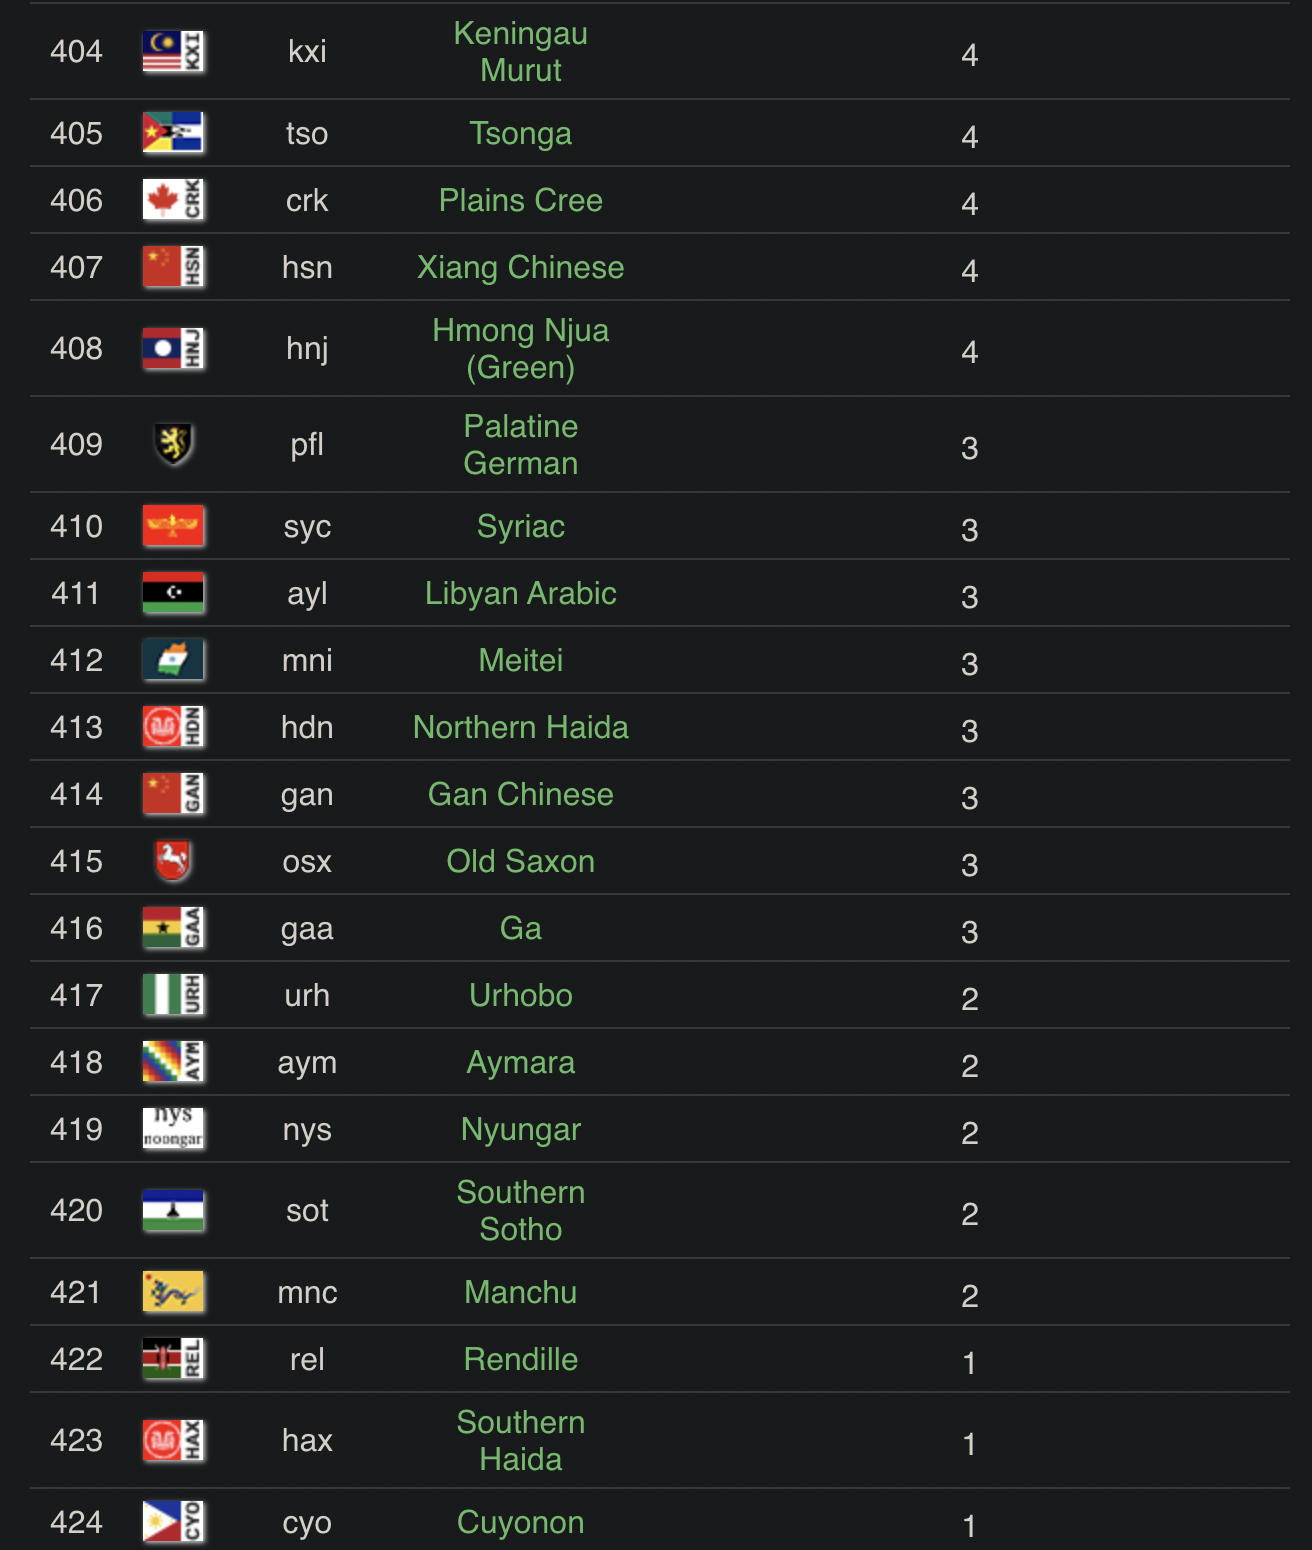
\includegraphics[width=0.46\linewidth]{images/tatoeba_bottom_20_lang.png}
    \caption{Tatoeba top 20 and bottom 20 languages based on sentences count \cite{tatoeba}}
    \label{fig:tatoeba_top_bottom_languages}
\end{figure}

Sentences typically consist of everyday phrases such as 'I have to go to sleep', 'That is intriguing', and 'Where do you live?' They may also include single-word exclamations like 'Speak!' or 'Look!' Additionally, multiple sentences such as 'You may write in any language you want. On Tatoeba, all languages are considered equal', and 'Guns don't kill people. People kill people' can be found inside the corpus. A few of them also include human names, 'Compare your answer with Tom's', 'Muiriel is 20 now'. All of the sentences are straightforward and literal, without the use of linguistic devices such as metaphors or sarcasm. Therefore, machine translation process should be straightforward on this level.

The languages chosen for evaluation in this study represent a wide overview, striking a balance between resources and diversity. Each language will then be translated into English (Many-to-English) and evaluated. The evaluation criteria encompass standard metrics such as BLEU (Bilingual Evaluation Understudy) \cite{papieni-2002-bleu}, METEOR (Metric for Evaluation of Translation with Explicit ORdering) \cite{lavie-2007-meteor} to capture nuances in translation quality. These metrics not only quantify the fidelity of translations but also offer insights into the models' adaptability and robustness across different linguistic pairs.

\begin{table}[htbp]
    \centering
    \begin{tabular}{|l|l|}
        \hline
        \textbf{No.} & \textbf{Language} \\
        \hline
        1            & Dutch             \\
        2            & Finnish           \\
        3            & French            \\
        4            & German            \\
        5            & Hebrew            \\
        6            & Hungarian         \\
        7            & Italian           \\
        8            & Japanese          \\
        9            & Mandarin Chinese  \\
        10           & Polish            \\
        11           & Portuguese        \\
        12           & Russian           \\
        13           & Spanish           \\
        14           & Turkish           \\
        15           & Ukrainian         \\
        \hline
    \end{tabular}
    \caption{List of chosen languages for evaluation}
\end{table}

Sentences dataset from Tatoeba is used \footnote{\url{https://tatoeba.org/}}. Languages that has more than fifty thousand sentences are selected. Accordingly, languages that are available for mbart is also selected based on the list here \footnote{\url{https://dl-translate.readthedocs.io/en/latest/available_languages/}}

For translation, all languages are translated into English as the target language. Then compare the true English sentence and the predicted one, calculated BLEU.

GPT-4 \cite{openai-2024-gpt4} try GPT and see

READ THIS \cite{intento-2020} (exactly what this paper should do, maybe compare results and find insights)

\section{Evaluation}

\section{Conclusion}

\printbibliography
\end{document}
